\section{Stabilität im Nyquist-Diagramm}

Die Idee des Nyquist-Kriteriums ist es, anhand der \textbf{Ortskurve} $H(s)$ \textbf{(offener Regelkreis)} einen Aussage über die
\textbf{Stabilität} des \textbf{(geschlossenen Regelkreises)} zu machen. \\
Ausserdem kann mittels \textbf{Amplitudenrand} und \textbf{Phasenrand} eine \textbf{relative Aussage} über die Stabilität
des Systems gemacht werden.


\subsection{Offener und geschlossener Regelkreis}

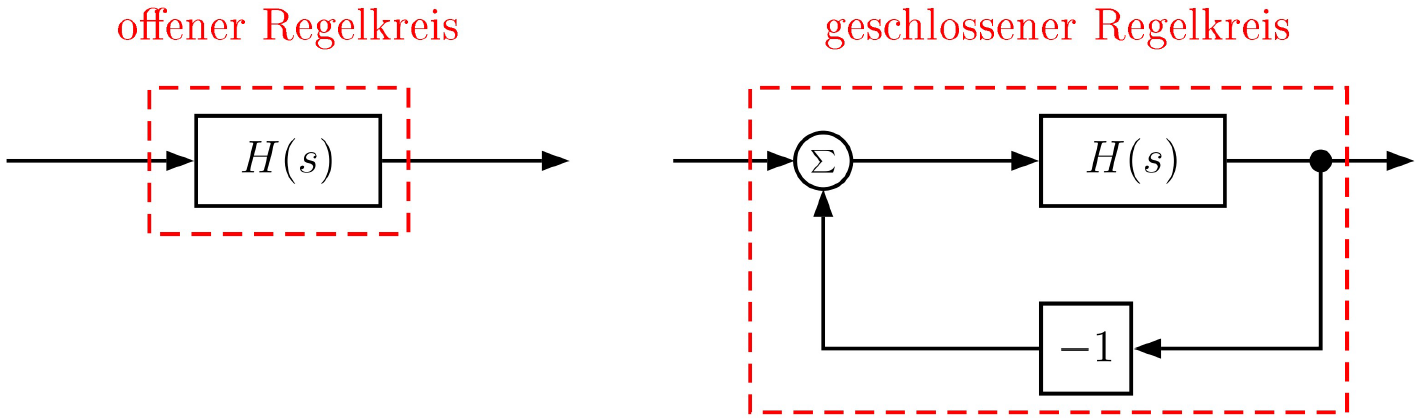
\includegraphics[width=0.75\columnwidth]{images/offener_geschlossener_regelkreis.png}

$$ H_{\text{geschlossen}(s)} = \frac{H(s)}{1 + H(s)} = \frac{N(s)}{D(s) + N(s)} $$


\subsection{Vereinfachtes Nyquist-Kriterium}

\fbox{\parbox{0.95\columnwidth}{
Ist der \textbf{offene} Regelkreis $H(s)$ \textbf{asymptotisch stabil} (alle Pole in der LHE), so ist der \textbf{geschlossene}
Regelkreis $\frac{H(s)}{1 + H(s)}$ asymptotisch stabil, wenn die \textbf{Ortskurve} des \textbf{offenen} Regelkreises den 
kritischen Punkt ($-1$, $\jimg 0$) mit wachsender Frequenz weder umkreist noch durchläuft, sondern '\textbf{links} liegen lässt'.
}}


\subsection{Amplitudenrand und Phasenrand (Verstärkungsreserve)}

Mit dem Amplitudenrand und dem Phasenrand kann ausgesagt werden, um wieviel entweder die \textbf{Verstäkung} oder die \textbf{Phase}
erhöht werden kann, bis der geschlossene Regelkreis \textbf{instabil} (bzw. \textbf{grenzstabil}) wird.

\begin{outline}
    \1 \textbf{Amplitudenrand (Verstärkungsreserve)}
        \2 Frequenz, bei welche die \textbf{negative} relle Achse geschnitten wird: $\omega_{\pi}$
        \2 Bei $\omega_{\pi}$: $\frac{1}{\text{Amplitudenrand}} =$ Abstand zum Ursprung
    \1 \textbf{Phasenrand (Phasenreserve)}
        \2 Frequenz, bei welche  Eintritt in den Einheitskreis erfolgt: $\omega_D$
        \2 Bei $\omega_D$: Winkel bis zu $180 \, \degree$   % TODO Bessere Formulierung?
\end{outline}


\subsection{Amplitudenrand und Phasenrand im Nyquist-Diagramm}

\begin{minipage}[c]{0.5\columnwidth}
    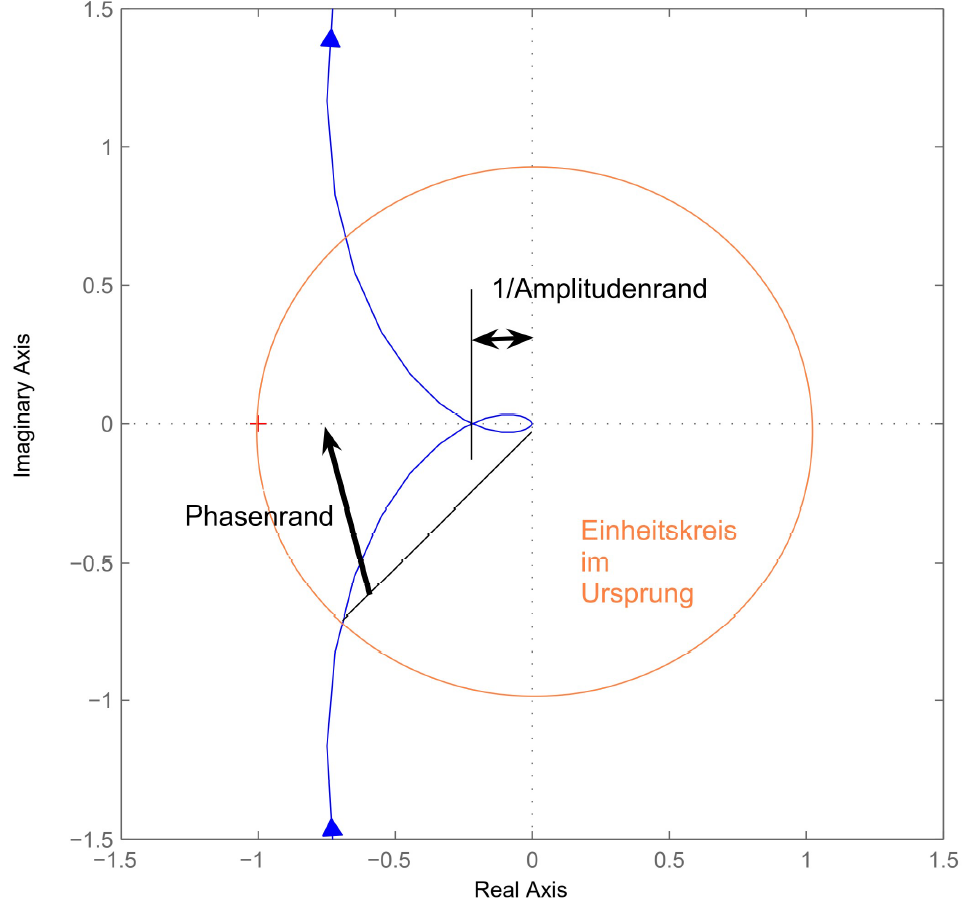
\includegraphics[width=\columnwidth]{images/nyquist_amplitudenrand_phasenrand.png}
\end{minipage}
\hfill
\begin{minipage}[c]{0.45\columnwidth}
    Das System ist \textbf{stabil}, da der kritische Punkt ($-1$, $\jimg 0$) '\textbf{links} liegen gelassen'
    wird, wenn man sich mit aufsteigender Frequenz auf der Ortskurve bewegt. \\

    Es kann auch argumentiert werden, dass das System stabil ist, da sowohl Amplitudenrand als auch Phasenrand $> 0$ sind.
\end{minipage}
